\nchapter{Übersichten}

\section{Silbenstruktur (\horenref{lands:syllable-structure})}
\begin{center}\footnotesize
	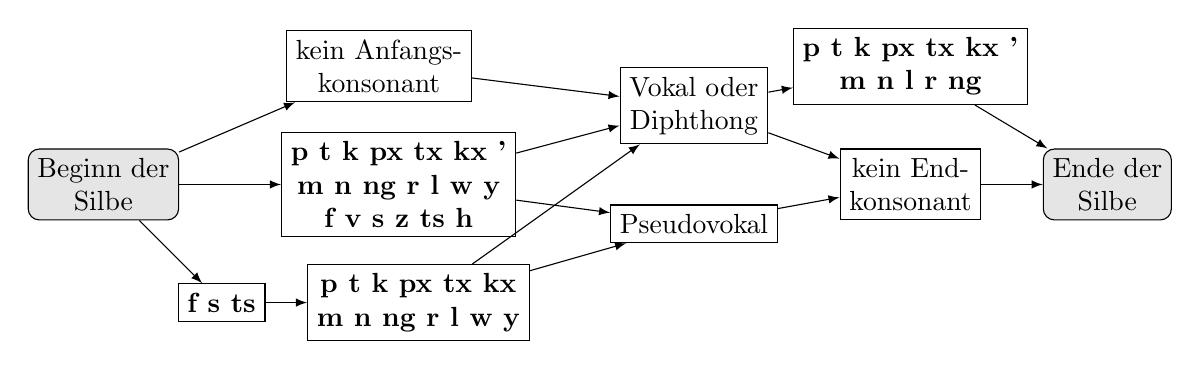
\begin{tikzpicture}[every path/.style={>=latex},every node/.style={draw,rectangle}]
		\node[rounded corners,fill=gray!20,align=center] (sos) at (-4,1) {Beginn der\\Silbe};
		\node[align=center] (zero-onset) at (-0.5,2.5) {kein Anfangs-\\konsonant};
		\node[align=center,font=\bfseries] (onset) at (-0.25,1) {p t k px tx kx '\\ m n ng r l w y\\f v s z ts h};
		\node[font=\bfseries] (clust-c1) at (-2.5,-0.5) {f s ts};
		\node[align=center,font=\bfseries] (clust-c2) at (0,-0.5) {p t k px tx kx\\m n ng r l w y};
		\node[align=center] (vowel) at (3.5,2) {Vokal oder\\Diphthong};
		\node (pseudovowel) at (3.5,0.5) {Pseudovokal};
		\node[align=center,font=\bfseries] (final) at (6.25,2.5) {p t k px tx kx ’\\m n l r ng};
		\node[align=center] (zero-coda) at (6.25,1) {kein End-\\konsonant};
		\node[rounded corners,fill=gray!20,align=center] (eos) at (8.75,1) {Ende der\\Silbe};
		
		\draw[->] (sos) edge (clust-c1);
		\draw[->] (sos) edge (onset);
		\draw[->] (sos) edge (zero-onset);
		\draw[->] (clust-c1) edge (clust-c2);
		\draw[->] (zero-onset) edge (vowel);
		\draw[->] (clust-c2) edge (vowel);
		\draw[->] (clust-c2) edge (pseudovowel);
		\draw[->] (onset) edge (vowel);
		\draw[->] (onset) edge (pseudovowel);
		\draw[->] (vowel) edge (final);
		\draw[->] (final) edge (eos);
		\draw[->] (vowel) edge (zero-coda);
		\draw[->] (pseudovowel) edge (zero-coda);
		\draw[->] (zero-coda) edge (eos);
	\end{tikzpicture}
\end{center}

\section{Fallendungen (\horenref{morph:decl})}
{\small
	\begin{center}
		\begin{tabular}{lccccccc}
			& Absolutiv & Agens & Patiens & Dativ & Genitiv & Topik & \\
			\hline 
			-a, -ä, -e, -i, -ì & --- & \N{-l} & \N{-t}, \N{-ti} & \N{-r}, \N{-ru} & \N{-yä} & \N{-ri} & \\
			-o & --- & \N{-l} & \N{-t}, \N{-ti} & \N{-r}, \N{-ru} & \N{-ä} & \N{-ri} & \\
			-u, (-ù \E{Riff-Na'vi}) & --- & \N{-l} & \N{-t}, \N{-ti} & \N{-r}, \N{-ru} & \N{-ä} & \N{-ri} & \\
			Konsonant / Pseudovokal & --- & \N{-ìl} & \N{-it}, \N{-ti} & \N{-ur} & \N{-ä} & \N{-ìri} & \\
			-ey & --- & \N{-ìl} & \N{-t}, \N{-ti} & \N{-ru}, \N{-ur} & \N{-ä} & \N{-ri} & \\
			-ay & --- & \N{-ìl} & \N{-t}, \N{-it}, \N{-ti} & \N{-ru}, \N{-ur} & \N{-ä} & \N{-ri} & \\
			-ew & --- & \N{-ìl} & \N{-it}, \N{-ti} & \N{-r}, \N{-ru} & \N{-ä} & \N{-ri} & \\
			-aw & --- & \N{-ìl} & \N{-it}, \N{-ti} & \N{-r}, \N{-ru}, \N{-ur} & \N{-ä} & \N{-ri} & \\
			’ (tìftang) & --- & \N{-ìl} & \N{-it}, \N{-ti} & \N{-ru}, \N{-ur} & \N{-ä} & \N{-ri}, \N{-ìri} & \\
\end{tabular}\end{center}}

\section{Reihenfolge der Nominalaffixe (\horenref{morph:prenoun:combination})}
\begin{center}
	\begin{tabular}{lccccccccc}
		\N{fì-} & & \N{ay+} (\N{fay+}, \N{tsay+}, \N{pay+}, \N{fray+}) & \N{fne-} & Sub- & & & & & Fall- \\
		\N{tsa-} & \N{fra-} & \N{me+} & \N{sna-} & stan- & \N{-fkeyk} & \N{-tsyìp} & \N{-o} & \N{-pe} & en- \\
		\N{pe+} & & \N{pxe+} (\N{pepe+}) & \N{munsna-} & tiv & & & & & dung
	\end{tabular}
\end{center}
\pagebreak

\section{Pronomina (\horenref{morph:pron}, \horenref{morph:hon-pron}, \horenref{morph:lahe:short}, \horenref{morph:correlatives}, \horenref{morph:questions})}
\subsection{1. Person exklusiv}
\begin{center}
	\begin{tabular}{lcccccc}
		& Absolutiv & Agens & Patiens & Dativ & Genitiv & Topik \\
		\hline
		Singular & \N{oe} & \N{oel} & \N{oet(i)} & \N{oer(u)} & \N{oey(ä)} & \N{oeri} \\
		Dual & \N{moe} & \N{moel} & \N{moet(i)} & \N{moer(u)} & \N{moey(ä)} & \N{moeri} \\
		Trial & \N{pxoe} & \N{pxoel} & \N{pxoet(i)} & \N{pxoer(u)} & \N{pxoey(ä)} & \N{pxoeri} \\
		Plural & \N{ayoe} & \N{ayoel} & \N{ayoet(i)} & \N{ayoer(u)} & \N{ayoey(ä)} & \N{ayoeri} \\ 
	\end{tabular} 
\end{center}

\subsection{1. Person exklusiv (zeremoniell)}
\begin{center}
	\begin{tabular}{lcccccc}
		& Absolutiv & Agens & Patiens & Dativ & Genitiv & Topik \\
		\hline
		Singular & \N{ohe} & \N{ohel} & \N{ohet(i)} & \N{oher(u)} & \N{oheyä} & \N{oheri} \\
		Dual & \N{mohe} & \N{mohel} & \N{mohet(i)} & \N{moher(u)} & \N{moheyä} & \N{moheri} \\
		Trial & \N{pxohe} & \N{pxohel} & \N{pxohet(i)} & \N{pxoher(u)} & \N{pxoheyä} & \N{pxoheri} \\
		Plural & \N{ayohe} & \N{ayohel} & \N{ayohet(i)} & \N{ayoher(u)} & \N{ayoheyä} & \N{ayoheri} \\ 
	\end{tabular} 
\end{center}

\subsection{1. Person inklusiv}
\begin{center}
	\begin{tabular}{lcccccc}
		& Absolutiv & Agens & Patiens & Dativ & Genitiv & Topik \\
		\hline
		Singular & --- & --- & --- & --- & --- & --- \\
		Dual & \N{oeng} & \N{oengal} & \N{oengat(i)} & \N{oengar(u)} & \N{oengey(ä)} & \N{oengari} \\
		Trial & \N{pxoeng} & \N{pxoengal} & \N{pxoengat(i)} & \N{pxoengar(u)} & \N{pxoengey(ä)} & \N{pxoengari} \\
		\multirow{2}{*}{Plural} & \N{ayoeng}, & \N{ayoengal}, & \N{ayoengat(i)}, & \N{ayoengar(u)}, & \N{ayoengey(ä)}, & \N{ayoengari}, \\
		& \N{awnga} & \N{awngal} & \N{awngat(i)} & \N{awngar(u)} & \N{awngey(ä)} & \N{awngari}
	\end{tabular} 
\end{center}

\subsection{1. Person inklusiv (zeremoniell)}
\begin{center}
	\begin{tabular}{lcccccc}
		& Absolutiv & Agens & Patiens & Dativ & Genitiv & Topik \\
		\hline
		Singular & --- & --- & --- & --- & --- & --- \\
		Dual & \N{oheng} & \N{ohengal} & \N{ohengat(i)} & \N{ohengar(u)} & \N{ohengeyä} & \N{ohengari} \\
		Trial & \N{pxoheng} & \N{pxohengal} & \N{pxohengat(i)} & \N{pxohengar(u)} & \N{pxohengeyä} & \N{pxohengari} \\
		Plural & \N{ayoheng} & \N{ayohengal} & \N{ayohengat(i)} & \N{ayohengar(u)} & \N{ayohengeyä} & \N{ayohengari}
	\end{tabular} 
\end{center}

\subsection{2. Person}
\begin{center}
	\begin{tabular}{lcccccc}
		& Absolutiv & Agens & Patiens & Dativ & Genitiv & Topik \\
		\hline
		Singular & \N{nga} & \N{ngal} & \N{ngat(i)} & \N{ngar(u)} & \N{ngey(ä)} & \N{ngari} \\
		Dual & \N{menga} & \N{mengal} & \N{mengat(i)} & \N{mengar(u)} & \N{mengey(ä)} & \N{mengari} \\
		Trial & \N{pxenga} & \N{pxengal} & \N{pxengat(i)} & \N{pxengar(u)} & \N{pxengey(ä)} & \N{pxengari} \\
		Plural & \N{aynga} & \N{ayngal} & \N{ayngat(i)} & \N{ayngar(u)} & \N{ayngey(ä)} & \N{ayngari} \\ 
	\end{tabular} 
\end{center}

\subsection{2. Person (zeremoniell)}
\begin{center}
	\begin{tabular}{lcccccc}
		& Absolutiv & Agens & Patiens & Dativ & Genitiv & Topik \\
		\hline
		Singular & \N{ngenga} & \N{ngengal} & \N{ngengat(i)} & \N{ngengar(u)} & \N{ngengeyä} & \N{ngengari} \\
		Dual & \N{mengenga} & \N{mengengal} & \N{mengengat(i)} & \N{mengengar(u)} & \N{mengengeyä} & \N{mengengari} \\
		Trial & \N{pxengenga} & \N{pxengengal} & \N{pxengengat(i)} & \N{pxengengar(u)} & \N{pxengengeyä} & \N{pxengengari} \\
		Plural & \N{ayngenga} & \N{ayngengal} & \N{ayngengat(i)} & \N{ayngengar(u)} & \N{ayngengeyä} & \N{ayngengari} \\ 
	\end{tabular} 
\end{center}

\subsection{3. Person belebt}
\begin{center}
	\begin{tabular}{lcccccc}
		& Absolutiv & Agens & Patiens & Dativ & Genitiv & Topik \\
		\hline
		Singular & \N{po} & \N{pol} & \N{pot(i)} & \N{por(u)} & \N{pey(ä)} & \N{pori} \\
		Dual & \N{mefo} & \N{mefol} & \N{mefot(i)} & \N{mefor(u)} & \N{mefey(ä)} & \N{mefori} \\
		Trial & \N{pxefo} & \N{pxefol} & \N{pxefot(i)} & \N{pxefor(u)} & \N{pxefey(ä)} & \N{pxefori} \\
		Plural & \N{(ay)fo} & \N{(ay)fol} & \N{(ay)fot(i)} & \N{(ay)for(u)} & \N{(ay)fey(ä)} & \N{(ay)fori} \\ 
	\end{tabular} 
\end{center}

\subsection{3. Person belebt (zeremoniell)}
\begin{center}
	\begin{tabular}{lcccccc}
		& Absolutiv & Agens & Patiens & Dativ & Genitiv & Topik \\
		\hline
		Singular & \N{poho} & \N{pohol} & \N{pohot(i)} & \N{pohor(u)} & \N{poheyä} & \N{pohori} \\
		Dual & \QUAESTIO{\N{mefoho}} & \QUAESTIO{\N{mefohol}} & \QUAESTIO{\N{mefohot(i)}} & \QUAESTIO{\N{mefohor(u)}} & \QUAESTIO{\N{mefoheyä}} & \QUAESTIO{\N{mefohori}} \\
		Trial & \QUAESTIO{\N{pxefoho}} & \QUAESTIO{\N{pxefohol}} & \QUAESTIO{\N{pxefohot(i)}} & \QUAESTIO{\N{pxefohor(u)}} & \QUAESTIO{\N{pxefoheyä}} & \QUAESTIO{\N{pxefohori}} \\
		Plural & \QUAESTIO{\N{(ay)foho}} & \QUAESTIO{\N{(ay)fohol}} & \QUAESTIO{\N{(ay)fohot(i)}} & \QUAESTIO{\N{(ay)fohor(u)}} & \QUAESTIO{\N{(ay)foheyä}} & \QUAESTIO{\N{(ay)fohori}} \\ 
	\end{tabular} 
\end{center}

\subsection{3. Person belebt (Maskulinum)}
\begin{center}
	\begin{tabular}{lcccccc}
		& Absolutiv & Agens & Patiens & Dativ & Genitiv & Topik \\
		\hline
		Singular & \N{poan} & \N{poanìl} & \N{poanit, poanti} & \N{poanur} & \N{poanä} & \N{poanìri} \\
	\end{tabular} 
\end{center}

\subsection{3. Person belebt (Maskulinum -- zeremoniell)}
\begin{center}
	\begin{tabular}{lcccccc}
		& Absolutiv & Agens & Patiens & Dativ & Genitiv & Topik \\
		\hline
		Singular & \N{pohan} & \N{pohanìl} & \N{pohanit, pohanti} & \N{pohanur} & \N{pohanä} & \N{pohanìri} \\
	\end{tabular} 
\end{center}

\subsection{3. Person belebt (Femininum)}
\begin{center}
	\begin{tabular}{lcccccc}
		& Absolutiv & Agens & Patiens & Dativ & Genitiv & Topik \\
		\hline
		Singular & \N{poe} & \N{poel} & \N{poet(i)} & \N{poer(u)} & \N{poey(ä)} & \N{poeri} \\
	\end{tabular} 
\end{center}

\subsection{3. Person belebt (Femininum -- zeremoniell)}
\begin{center}
	\begin{tabular}{lcccccc}
		& Absolutiv & Agens & Patiens & Dativ & Genitiv & Topik \\
		\hline
		Singular & \N{pohe} & \N{pohel} & \N{pohet(i)} & \N{poher(u)} & \N{poheyä} & \N{poheri} \\
	\end{tabular} 
\end{center}

\subsection{3. Person unbelebt}
\begin{center}
	\begin{tabular}{lcccccc}
		& Absolutiv & Agens & Patiens & Dativ & Genitiv & Topik \\
		\hline
		\multirow{2}{*}{Singular} & \N{tsa'u}, & \N{tsa'ul}, & \N{tsa'ut(i)}, & \N{tsa'ur(u)}, & \QUAESTIO{\N{tsa'uä}}, & \N{tsa'uri}, \\
		& \N{tsaw} & \N{tsal} & \N{tsat(i)} & \N{tsar(u)} & \N{tsey(ä)} & \N{tsari} \\
		\multirow{2}{*}{Dual} & \N{mesa'u}, & \N{mesa'ul}, & \N{mesa'ut(i)}, & \N{mesa'ur(u)}, & \QUAESTIO{\N{mesa'uä}}, & \N{mesa'uri}, \\
		& \N{mesaw} & \N{mesal} & \N{mesat(i)} & \N{mesar(u)} & \N{mesey(ä)} & \N{mesari} \\
		\multirow{2}{*}{Trial} & \N{pxesa'u}, & \N{pxesa'ul}, & \N{pxesa'ut(i)}, & \N{pxesa'ur(u)}, & \QUAESTIO{\N{pxesa'uä}}, & \N{pxesa'uri}, \\
		& \N{pxesaw} & \N{pxesal} & \N{pxesat(i)} & \N{pxesar(u)} & \N{pxesey(ä)} & \N{pxesari} \\
		\multirow{2}{*}{Plural} & \N{(ay)sa'u}, & \N{(ay)sa'ul}, & \N{(ay)sa'ut(i)}, & \N{(ay)sa'ur(u)}, & \QUAESTIO{\N{(ay)sa'uä}}, & \N{(ay)sa'uri}, \\
		& \N{(ay)saw} & \N{(ay)sal} & \N{(ay)sat(i)} & \N{(ay)sar(u)} & \N{(ay)sey(ä)} & \N{(ay)sari} \\
		\end{tabular}
	\end{center} \label{tables:3rdPerson:inanimate}

\subsection{Unpersönliches Pronomen}
\begin{center}
	\begin{tabular}{lcccccc}
		& Absolutiv & Agens & Patiens & Dativ & Genitiv & Topik \\
		\hline
		Singular & \N{fko} & \N{fkol} & \N{fkot(i)} & \N{fkor(u)} & \N{fkey(ä)} & \N{fkori} \\
	\end{tabular} 
\end{center}

\subsection{Reflexivpronomen}
\begin{center}
	\begin{tabular}{lcccccc}
		& Absolutiv & Agens & Patiens & Dativ & Genitiv & Topik \\
		\hline
		Singular & \N{sno} & --- & --- & \N{snor(u)} & \N{sney(ä)} & \N{snori} \\
	\end{tabular} 
\end{center}

\subsection{Indefinitpronomen}
\subsubsection{} \N{frapo} \E{jede/r}
\begin{center}
	\begin{tabular}{lcccccc}
		& Absolutiv & Agens & Patiens & Dativ & Genitiv & Topik \\
		\hline
		Singular & \N{frapo} & \N{frapol} & \N{frapot(i)} & \N{frapor(u)} & \N{frapey(ä)} & \N{frapori} \\
	\end{tabular} 
\end{center}

\subsubsection{} \N{fra'u} \E{alles (Sache)}
\begin{center}
	\begin{tabular}{lcccccc}
		& Absolutiv & Agens & Patiens & Dativ & Genitiv & Topik \\
		\hline
		Singular & \N{fra'u} & \N{fra'ul} & \N{fra'ut(i)} & \N{fra'ur(u)} & \N{fra'uä} & \N{fra'uri} \\
	\end{tabular} 
\end{center}

\subsubsection{} \QUAESTIO{\N{frakem} \E{alles (Aktion)}}
\begin{center}
	\begin{tabular}{lcccccc}
		& Absolutiv & Agens & Patiens & Dativ & Genitiv & Topik \\
		\hline
		Singular & \QUAESTIO{\N{frakem}} & \QUAESTIO{\N{frakemìl}} & \QUAESTIO{\N{frakemit}, \N{frakemti}} & \QUAESTIO{\N{frakemur(u)}} & \QUAESTIO{\N{frakemä}} & \QUAESTIO{\N{frakemìri}} \\
	\end{tabular} 
\end{center}

\subsubsection{} \N{kawtu} \E{niemand}
\begin{center}
	\begin{tabular}{lcccccc}
		& Absolutiv & Agens & Patiens & Dativ & Genitiv & Topik \\
		\hline
		Singular & \N{kawtu} & \N{kawtul} & \N{kawtut(i)} & \N{kawtur(u)} & \N{kawtuä} & \N{kawturi} \\
	\end{tabular} 
\end{center}

\subsubsection{} \N{ke'u} \E{nichts (Sache)}
\begin{center}
	\begin{tabular}{lcccccc}
		& Absolutiv & Agens & Patiens & Dativ & Genitiv & Topik \\
		\hline
		Singular & \N{ke'u} & \N{ke'ul} & \N{ke'ut(i)} & \N{ke'ur(u)} & \N{ke'uä} & \N{ke'uri} \\
	\end{tabular} 
\end{center}

\subsubsection{} \N{kekem} \E{nichts (Aktion)}
\begin{center}
	\begin{tabular}{lcccccc}
		& Absolutiv & Agens & Patiens & Dativ & Genitiv & Topik \\
		\hline
		Singular & \N{kekem} & \QUAESTIO{\N{kekemìl}} & \QUAESTIO{\N{kekemit}, \N{kekemti}} & \QUAESTIO{\N{kekemur(u)}} & \QUAESTIO{\N{kekemä}} & \QUAESTIO{\N{kekemìri}} \\
	\end{tabular} 
\end{center}

\subsubsection{} \N{lahe} \E{andere/r/s}
\begin{center}
	\begin{tabular}{lcccccc}
		& Absolutiv & Agens & Patiens & Dativ & Genitiv & Topik \\
		\hline
		\multirow{2}{*}{Singular} & \N{lahe}, & \N{lahel}, & \N{lahet(i)}, & \N{laher(u)}, & \N{lahey(ä)}, & \N{laheri}, \\
		& \N{lapo} & \N{lapol} & \N{lapot(i)} & \N{lapor(u)} & \N{lapey(ä)} & \N{lapori} \\
		Dual & \QUAESTIO{\N{melahe}} & \QUAESTIO{\N{melahel}} & \QUAESTIO{\N{melahet(i)}} & \QUAESTIO{\N{melaher(u)}} & \QUAESTIO{\N{melahey(ä)}} & \QUAESTIO{\N{melaheri}} \\
		Trial & \QUAESTIO{\N{pxelahe}} & \QUAESTIO{\N{pxelahel}} & \QUAESTIO{\N{pxelahet(i)}} & \QUAESTIO{\N{pxelaher(u)}} & \QUAESTIO{\N{pxelahey(ä)}} & \QUAESTIO{\N{pxelaheri}} \\
		\multirow{2}{*}{Plural} & \N{aylahe}, & \N{aylahel}, & \N{aylahet(i)}, & \N{aylaher(u)}, & \N{aylahey(ä)}, & \N{aylaheri}, \\
		& \N{ayla} & \N{aylal} & \N{aylat(i)} & \N{aylar(u)} & \N{ayley(ä)} & \N{aylari}
	\end{tabular} 
\end{center}

\subsection{Demonstrativpronomina}
\subsubsection{} \N{fìpo} \E{diese Person}
\begin{center}
	\begin{tabular}{lcccccc}
		& Absolutiv & Agens & Patiens & Dativ & Genitiv & Topik \\
		\hline
		Singular & \N{fìpo} & \N{fìpol} & \N{fìpot(i)} & \N{fìpor(u)} & \N{fìpey(ä)} & \N{fìpori} \\
	\end{tabular} 
\end{center}

\subsubsection{} \N{fì'u} \E{diese/r/s (Sache)}
\begin{center}
	\begin{tabular}{lcccccc}
		& Absolutiv & Agens & Patiens & Dativ & Genitiv & Topik \\
		\hline
		Singular & \N{fì'u} & \N{fì'ul} & \N{fì'ut(i)} & \N{fì'ur(u)} & \N{fì'uä} & \N{fì'uri} \\
	\end{tabular} 
\end{center}

\subsubsection{} \N{fìkem} \E{dies (Aktion)}
\begin{center}
	\begin{tabular}{lcccccc}
		& Absolutiv & Agens & Patiens & Dativ & Genitiv & Topik \\
		\hline
		Singular & \N{fìkem} & \N{fìkemìl} & \N{fìkemit}, \N{fìkemti} & \N{fìkemur} & \N{fìkemä} & \N{fìkemìri} \\
	\end{tabular} 
\end{center}

\subsubsection{} \N{tsapo}, \N{tsatu} \E{jene Person}
\begin{center}
	\begin{tabular}{lcccccc}
		& Absolutiv & Agens & Patiens & Dativ & Genitiv & Topik \\
		\hline
		\multirow{2}{*}{Singular} & \N{tsapo}, & \N{tsapol}, & \N{tsapot(i)}, & \N{tsapor(u)}, & \N{tsapey(ä)}, & \N{tsapori}, \\
		& \N{tsatu} & \N{tsatul} & \N{tsatut(i)} & \N{tsatur(u)} & \N{tsatuä} & \N{tsaturi} \\
		\multirow{2}{*}{Dual} & \QUAESTIO{\N{mesapo}}, & \QUAESTIO{\N{mesapol}}, & \QUAESTIO{\N{mesapot(i)}}, & \QUAESTIO{\N{mesapor(u)}}, & \QUAESTIO{\N{mesapey(ä)}}, & \QUAESTIO{\N{mesapori}}, \\
		& \QUAESTIO{\N{mesatu}} & \QUAESTIO{\N{mesatul}} & \QUAESTIO{\N{mesatut(i)}} & \QUAESTIO{\N{mesatur(u)}} & \QUAESTIO{\N{mesatuä}} & \QUAESTIO{\N{mesaturi}} \\
		\multirow{2}{*}{Trial} & \QUAESTIO{\N{pxesapo}}, & \QUAESTIO{\N{pxesapol}}, & \QUAESTIO{\N{pxesapot(i)}}, & \QUAESTIO{\N{pxesapor(u)}}, & \QUAESTIO{\N{pxesapey(ä)}}, & \QUAESTIO{\N{pxesapori}}, \\
		& \QUAESTIO{\N{pxesatu}} & \QUAESTIO{\N{pxesatul}} & \QUAESTIO{\N{pxesatut(i)}} & \QUAESTIO{\N{pxesatur(u)}} & \QUAESTIO{\N{pxesatuä}} & \QUAESTIO{\N{pxesaturi}} \\
		\multirow{2}{*}{Plural} & \QUAESTIO{\N{(ay)sapo}}, & \QUAESTIO{\N{(ay)sapol}}, & \QUAESTIO{\N{(ay)sapot(i)}}, & \QUAESTIO{\N{(ay)sapor(u)}}, & \QUAESTIO{\N{(ay)sapey(ä)}}, & \QUAESTIO{\N{(ay)sapori}}, \\
		& \QUAESTIO{\N{(ay)satu}} & \QUAESTIO{\N{(ay)satul}} & \QUAESTIO{\N{(ay)satut(i)}} & \QUAESTIO{\N{(ay)satur(u)}} & \QUAESTIO{\N{(ay)satuä}} & \QUAESTIO{\N{(ay)saturi}} \\
	\end{tabular} 
\end{center}

\subsubsection{} \N{tsa'u} \E{jene/r/s (Sache)} -- s. \horenref{tables:3rdPerson:inanimate} 

\subsubsection{} \N{tsakem} \E{jenes (Aktion)}
\begin{center}
	\begin{tabular}{lcccccc}
		& Absolutiv & Agens & Patiens & Dativ & Genitiv & Topik \\
		\hline
		Singular & \N{tsakem} & \N{tsakemìl} & \N{tsakemit}, \N{tsakemti} & \N{tsakemur} & \N{tsakemä} & \N{tsakemìri} \\
	\end{tabular} 
\end{center}

\subsection{Interrogativpronomina}
\begin{center}
	\begin{tabular}{rlrl}
		Person & \N{pe\ACC{su}}, \N{\ACC{tu}pe} \E{wer?} & Sache & \N{pe\ACC{u}}, \N{\ACC{'u}pe} \E{was (welche Sache)?} \\
		Aktion & \N{pe\ACC{hem}}, \N{\ACC{kem}pe} \E{was (welche Aktion)?} & Zeit & \N{pe\ACC{hrr}}, \N{\ACC{krr}pe} \E{wann?} \\
		Ort & \N{pe\ACC{seng}}, \N{\ACC{tseng}pe} \E{wo?} & Art und Weise & \N{pe\ACC{fya}}, \N{\ACC{fya}pe} \E{wie?} \\
		Grund & \N{pe\ACC{lun}}, \N{\ACC{lum}pe} \E{warum?} & Typ & \N{pe\ACC{fnel}}, \N{\ACC{fne}pe} \E{welche Art?}\\
	\end{tabular}
\end{center}

\subsubsection{} Formen von \N{pesu} \E{wer?} und \N{pehem} \E{welche Handlung?}
\begin{center}
	\begin{tabular}{lccc}
		& Unspezifisch & Maskulinum & Femininum \\
		\hline
		Singular & \N{pe\ACC{su}}, \N{\ACC{tu}pe} & 
		\N{pe\ACC{stan}}, \N{tu\ACC{tam}pe} &
		\N{pe\ACC{ste}}, \N{tu\ACC{te}pe} \\
		Dual     & \N{pem\ACC{su}}, \N{me\ACC{su}pe} & 
		\N{pem\ACC{stan}}, \N{me\ACC{stam}pe} &
		\N{pem\ACC{ste}}, \N{me\ACC{ste}pe} \\
		Trial    & \N{pep\ACC{su}}, \N{pxe\ACC{su}pe} & 
		\N{pep\ACC{stan}}, \N{pxe\ACC{stam}pe} &
		\N{pep\ACC{ste}}, \N{pxe\ACC{ste}pe} \\
		Plural   & \N{pay\ACC{su}}, \N{(ay)\ACC{su}pe} & 
		\N{pay\ACC{stan}}, \N{(ay)\ACC{stam}pe} &
		\N{pay\ACC{ste}}, \N{(ay)\ACC{ste}pe} \\
	\end{tabular}
	\hskip2em
	\begin{center}
		\begin{tabular}{lc}
			Singular & \N{pe\ACC{hem}}, \N{\ACC{kem}pe} \\
			Dual & \N{pem\ACC{hem}}, \N{me\ACC{hem}pe} \\
			Trial & \N{pep\ACC{hem}}, \N{pxe\ACC{hem}pe} \\
			Plural & \N{pay\ACC{hem}}, \N{(ay)\ACC{hem}pe} \\
		\end{tabular}
	\end{center}
\end{center}

\section{Adverbiale Präfigierungen (\horenref{morph:correlatives})}
\begin{center}\small
	\begin{tabular}{rllllll}
		& Zeit & Ort & Art und Weise \\
		\hline
		\multirow{2}{*}{dies} & \N{set} & \N{fì\ACC{tseng}(e)} & \N{fì\ACC{fya}} \\ 
		& \E{jetzt} &  \E{hier} & \E{so, auf diese Weise} \\
		\multirow{2}{*}{jenes} & \N{tsa\ACC{krr}} & \N{tsatseng} & \N{\ACC{tsa}fya} \\
		& \E{dann} & \E{dort} & \E{auf jene Weise} \\
		\multirow{2}{*}{alle} & \N{\ACC{fra}krr} & \N{\ACC{fra}tseng} & \N{\ACC{fra}fya} \\
		& \E{immer} & \E{überall} & \E{in jeder Weise} \\
		\multirow{2}{*}{kein} & \N{\ACC{kaw}krr} & \N{\ACC{kaw}tseng} & --- \\
		& \E{nie} & \E{nirgends} \\
	\end{tabular}
\end{center}

\section{Desubstantivische Konjunktionen (\horenref{syn:attr:takrra}, \horenref{morph:fwa-tsawa})}
\subsection{Konjunktionen für Adverbialsätze}
\begin{center}
	\begin{tabular}{rlll}
		& am Anfang & am Ende \\
		\hline
		\E{nach} & \N{mawkrra} & \N{akrrmaw} & aus \N{maw krr a} \\
		\E{weil} & \N{talun(a)} & \N{alunta} & aus \N{ta lun a} \\
		\E{weil} & \N{taweyk(a)} & \QUAESTIO{\N{aweykta}} & aus \N{ta oeyk a}\\
		\E{wenn} & \N{krra} & \N{a krr} \\
		\E{dass} (als Ergebnis) & \N{kuma} & \N{akum} \\
		\E{seit} (ab dem Zeitpunkt) & \N{takrra} & \N{akrrta} & aus \N{ta krr a}\\
	\end{tabular}
\end{center}

\subsection{Konjunktionen für Inhaltssätze}
\begin{center}
	\begin{tabular}{rccc}
		Kasus & \N{fì'u}-Kontraktion & \N{tsa'u}-Kontraktion & \N{tì'eyng}-Kontraktion \\
		\hline
		Absolutiv & \N{fwa} ($<$ \N{fì'u a}) & \N{\ACC{tsa}wa} ($<$ \N{tsa'u a}) & \N{\ACC{teyng}a} ($<$ \N{tì'eyng a}) \\
		Agens & \N{\ACC{fu}la} ($<$ \N{fì'ul a}) & \N{\ACC{tsa}la} ($<$ \N{tsa'ul a}) & \N{\ACC{teyng}la} ($<$ \N{tì'eyngìl a}) \\
		Patiens & \N{\ACC{fu}ta} ($<$ \N{fì'ut a}) & \N{\ACC{tsa}ta} ($<$ \N{tsa'ut a}) & \N{\ACC{teyng}ta} ($<$ \N{tì'eyngit a}) \\
		Dativ & \N{\ACC{fu}ra} ($<$ \N{fì'ur a}) & \N{\ACC{tsa}ra} ($<$ \N{tsa'ur a}) & \N{\ACC{teyng}ra} ($<$ \N{tì'eyngur a}) \\
		Genitiv & --- & --- & \N{\ACC{teyng}ä} ($<$ \N{tì'eyngä a}) \\ 
		Topik & \N{\ACC{fu}ria} ($<$ \N{fì'uri a}) & \N{\ACC{tsa}ria} ($<$ \N{tsa'uri a}) & \N{\ACC{teyng}ria} ($<$ \N{tì'eyngìri a})\\
	\end{tabular}
\end{center} 
Die Substantive \N{fmawn} \E{Nachricht}, \N{faylì'u} \E{diese Worte} und \N{tson} \E{Pflicht, Verpflichtung} bilden Konjunktionen für Inhaltssätze nur im Patiens: \N{fmawnta} ($<$ \N{fmawnit a}), \N{fayluta} ($<$ \N{faylì'ut a}) und \N{tsonta} ($<$ \N{tsonit a}).

\pagebreak

\section{Infixe (\horenref{morph:infix:positions})}
\begin{center}
	\begin{tabular}{c|c|cc|cc|cccccc|cc|cc}
		\multicolumn{2}{c|}{Position 0} & \multicolumn{12}{c}{Position 1} & \multicolumn{2}{|c}{Position 2} \\
		\hline
		Reflexiv & Kausativ & \multicolumn{4}{|c|}{Tempus} & \multicolumn{6}{c}{Subjunktiv} & \multicolumn{2}{|c}{Aspekt} & \multicolumn{2}{|c}{Affekt} \\
		\cline{3-6} \cline{13-16}
		\N{\INF{äp}} & \N{\INF{eyk}} & \multicolumn{2}{|c|}{Vergangenheit} & \multicolumn{2}{|c|}{Zukunft} & \multicolumn{6}{c|}{\N{\INF{iv}}} & Imperfekt & Perfekt & Positiv & Negativ \\
		\cline{1-6} 
		\multicolumn{2}{c|}{Reflexiv + Kausativ} & Nah & Fern & Nah & Fern & & & & & & & \N{\INF{er}} & \N{\INF{ol}} & \N{\INF{ei}} & \N{\INF{äng}}\\
		\cline{15-16}
		\multicolumn{2}{c|}{\N{\INF{äpeyk}}} & \N{\INF{ìm}} & \N{\INF{am}} & \N{\INF{ìy}} & \N{\INF{ay}} & & & & & & & & & \multicolumn{2}{c}{Suppositiv} \\
		\cline{3-14}
		\multicolumn{2}{c|}{} & \multicolumn{7}{c|}{Tempus + Subjunktiv} & \multicolumn{5}{c|}{Subjunktiv + Aspekt} & \multicolumn{2}{c}{\N{\INF{ats}}} \\
		\cline{15-16}
		\multicolumn{2}{c|}{} & \multicolumn{7}{c|}{\N{\INF{imv}}, \N{\INF{ìyev}}, \N{\INF{iyev}}} & \multicolumn{5}{c|}{\N{\INF{irv}}, \N{\INF{ilv}}} & \multicolumn{2}{c}{Zeremoniell} \\
		\cline{3-14}
		\multicolumn{2}{c|}{} & \multicolumn{12}{c|}{Tempus + Aspekt} & \multicolumn{2}{c}{\N{\INF{uy}}} \\
		\multicolumn{2}{c|}{} & \multicolumn{12}{c|}{\N{\INF{ìrm}}, \N{\INF{ìry}}, \N{\INF{ìlm}}, \N{\INF{ìly}}} & & \\
		\multicolumn{2}{c|}{} & \multicolumn{12}{c|}{\N{\INF{arm}}, \N{\INF{ary}}, \N{\INF{alm}}, \N{\INF{aly}}} & & \\
		\cline{3-14}
		\multicolumn{2}{c|}{} & \multicolumn{7}{c|}{Zukunft + Absicht} & \multicolumn{5}{c|}{Partizip} & & \\
		\multicolumn{2}{c|}{} & \multicolumn{7}{c|}{\N{\INF{ìsy}}, \N{\INF{asy}}} & \multicolumn{5}{c|}{\N{\INF{us}}, \N{\INF{awn}}} & & \\
	\end{tabular} 
\end{center}

\section{Wahrnehmung (\horenref{semantics:percep})}
\begin{center}
	\begin{tabular}{c|ccccc}
		& \I{vtr} & \I{vtr} & \I{vin} & \I{n} & \I{n} \\
		& -Kontrolle & +Kontrolle & +Kontrolle & Empfindung & Fähigkeit \\
		\hline
		\multirow{2}{*}{sehen} & \N{tse'a}  & \N{nìn}  & \N{tìng nari}  & \N{'ur}  & \N{tse'atswo}  \\
		& {\scriptsize\E{sehen, erblicken}} & {\scriptsize\E{ansehen, hinsehen}} & {\scriptsize\E{ansehen, hinsehen}} & {\scriptsize\E{Aussehen}} & {\scriptsize\E{Sehvermögen}} \\
		\multirow{2}{*}{hören} & \N{stawm}  & \N{yune}  & \N{tìng mikyun}  & \N{pam} & \N{stawmtswo} \\
		& {\scriptsize\E{hören}} & {\scriptsize\E{zuhören}} & {\scriptsize\E{zuhören}} & {\scriptsize\E{Geräusch}}  & {\scriptsize\E{Hörvermögen, Gehör}} \\
		\multirow{2}{*}{riechen} & \N{hefi}  & \N{syam}  & \N{tìng ontu}  & \N{fahew}  & \N{hefitswo}  \\
		& {\scriptsize\E{riechen}} & {\scriptsize\E{riechen}} & {\scriptsize\E{riechen}} & {\scriptsize\E{Geruch}} & {\scriptsize\E{Geruchsvermögen}} \\
		\multirow{2}{*}{schmecken} & \N{ewku}  & \N{may'}  & \N{tìng ftxì}  & \N{sur}  & \N{ewktswo}  \\
		& {\scriptsize\E{schmecken}} & {\scriptsize\E{schmecken}} & {\scriptsize\E{schmecken}} & {\scriptsize\E{Geschmack, Aroma}} & {\scriptsize\E{Geschmackssinn}} \\
		\multirow{2}{*}{fühlen} & \N{zìm}  & \N{'ampi}  & \N{tìng zekwä}  & \N{zir}  & \N{zìmtswo}  \\
		& {\scriptsize\E{fühlen, anfühlen}} & {\scriptsize\E{berühren, anfassen}} & {\scriptsize\E{berühren, anfassen}} & {\scriptsize\E{Berührung, Gefühl}} & {\scriptsize\E{Tastsinn}}
	\end{tabular}
\end{center}